% arara: lualatex: { shell: true }
% arara: latexmk: { clean: partial }
\documentclass[class=book, crop=false, oneside, 12pt]{standalone}
\usepackage{standalone}
\usepackage{../../style}
\usepackage{../../glossary}

\let\isCompiledFromMain\undefined
\usepackage{../../music-tools}

\graphicspath{{./assets/images/}}
\ifdefined\isCompiledFromMain
\else
    \setluaoption{ly}{includepaths}{./assets/scores/}
\fi

\begin{document}

    \chapter{Sheep}
    \label{ch:04-sheep}

    Scegliere un secondo brano tra \acrshort{d}, \acrshort{p} e \acrshort{s} non è stato semplice. Si tratta di tre pezzi dall'elevato valore musicale e artistico in senso lato, ma anche di tre brani che hanno caratteristiche molto diverse tra loro; al netto delle preferenze personali\footnote{In anfratti remoti di internet si possono trovare disquisizioni piuttosto accese, ad esempio qui: \url{https://www.reddit.com/r/pinkfloyd/comments/8g9rk3/dogs_vs_pigs_vs_sheep/}},nessuno dei tre spicca sugli altri in assoluto, bensì ciascuno di essi ha caratteristiche che li rendono riconoscibili e meritevoli di analisi.

    Alla fine la scelta è caduta su \acrshort{s}. Ci sono molte ragioni che potrei menzionare in favore di questa scelta: tra le tante, il fatto che rappresenti il climax narrativo dell'album. Ma la ragione, in fin dei conti, è una sola: il solo di Rhodes iniziale di Wright. Semplicemente, non ho saputo resistere alla semplicità e al calore di un assolo dalla voce a metà tra il bluesy e il dorico che parla attraverso il timbro setoso del Mk I. Non poteva essere più azzeccato di così.

    In Sez.\ref{sec:04-intro} vengono introdotti il brano e le sue generalità. In Sez.\ref{sec:04-struttura} si parla della struttura del brano, proponendo una suddivisione in sezioni e una guida all'ascolto per ciascuna di esse. In Sez.\ref{sec:04-arrangement} sono approfondite alcune note di arrangiamento e composizione  del brano. In Sez.\ref{sec:04-harmony} sono proposte un'analisi e interpretazione armonica del brano, con particolare attenzione all'impianto narrativo.

    \section{Introduzione}
    \label{sec:04-intro}

    \acrlong{s} è la penultima traccia di \acrshort{anm}, ultima se consideriamo solo i tre brani core dell'album. 
    Il brano si sviluppa a partire da \emph{Raving and Drooling}, una composizione precedentemente utilizzata come base per improvvisazioni durante le esibizioni dal vivo della band a partire dal 1974. La registrazione definitiva fu realizzata tra aprile e luglio 1976 presso i \emph{Britannia Row Studios} di Londra~\cite{mabbett2010pink}. Un elemento distintivo del brano è l'inversione dei ruoli tra Gilmour e Waters, che suonano rispettivamente il basso e la chitarra; durante l'In The Flesh Tour, i due musicisti condividevano le parti di chitarra, mentre il basso era affidato al turnista Snowy White.

    Si tratta di una lunga suite della durata di dieci minuti, caratterizzata da sezioni eterogenee sia dal punto di vista armonico che ritmico. L'arrangiamento è ricco e stratificato: il basso 
    mantiene un ritmo swing costante; le chitarre, alternano groove, riff incisivi e tappeti ambientali; l'organo fornisce un sostegno armonico continuo, mentre campionamenti di animali e l'uso del vocoder arricchiscono il tessuto sonoro del brano.

    Dal punto di vista lirico, il brano è fortemente narrativo e racconta la storia delle pecore, metafora di soggetti sociali comandati dai cani. Le pecore vivono in uno stato d'inquietudine costante, incapaci d'identificare la fonte del loro malessere. Nel corso del brano, tuttavia, le pecore si liberano e si ribellano ai loro oppressori, solo per poi assumere esse stesse il ruolo dei cani, in un ciclo di oppressione apparentemente senza fine.

    \section{Struttura}
    \label{sec:04-struttura}

    Il brano si può dividere in \emph{quattro} sezioni principali.
    La suddivisione del brano in sezioni si basa su criteri che individuano similitudini intra-segmento e differenze extra-segmento; in particolare, le caratteristiche principali tenute in considerazione sono dinamica, tonalità e modo, progressione di accordi, voci impiegate e trame melodiche.

    Per comodità di consultazione, in questa analisi chiamiamo le quattro sezioni rispettivamente \songSec{A}, \songSec{B}, \songSec{C} e \songSec{D}, disposte nella conformazione \emph{ABCABD}. Il diagramma in Figura~\ref{fig:04-sections-timeline} mostra la posizione dei confini tra le sezioni individuate.

    \begin{figure}[htb]
        \centering
        \subimport{assets/figures}{sections_timeline.tex}
        \caption[Durata delle varie sezioni del brano.]{Durata delle varie sezioni del brano. In evidenza la struttura del brano: ABCABD.}
        \label{fig:04-sections-timeline}
    \end{figure}

    \begin{figure}[htb]
        \centering
        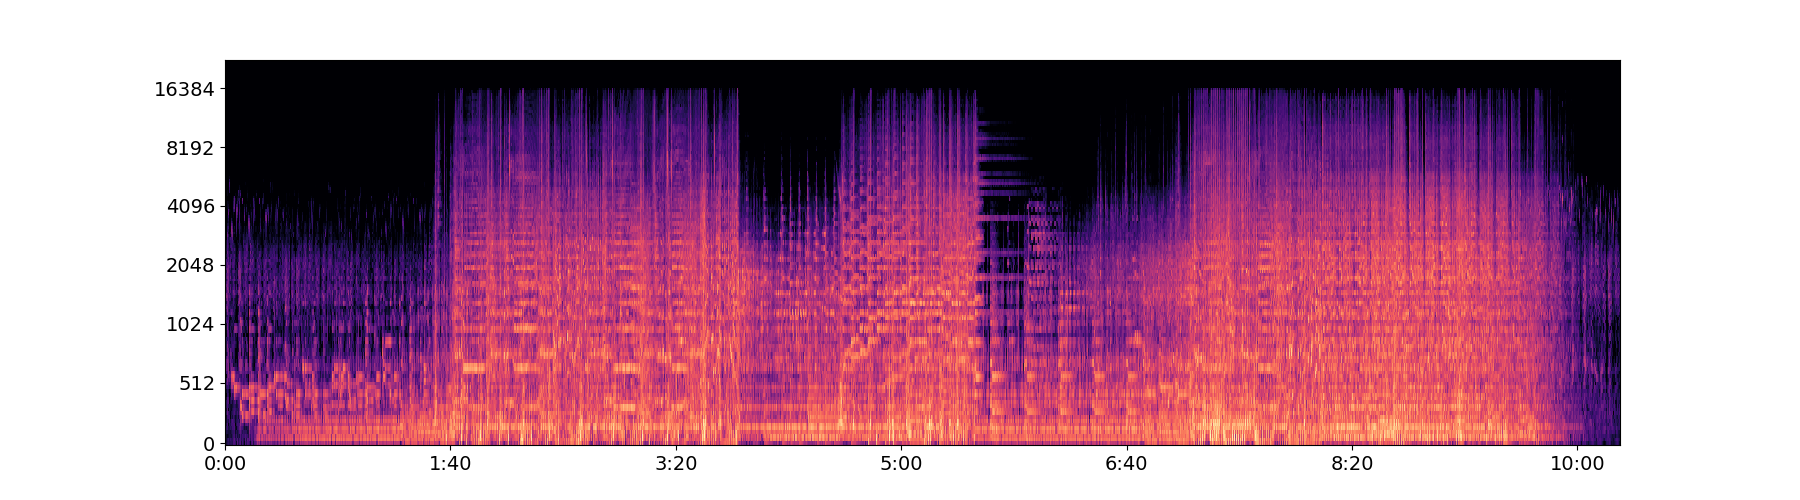
\includegraphics[width=\textwidth]{sheep_spectrogram.png}
        \caption[Spettrogramma rappresentante l'intero brano nel dominio delle frequenze.]{Spettrogramma rappresentante l'intero brano nel dominio delle frequenze. Il colore indica l'energia relativa per un momento della canzone in una banda di frequenza. È facile individuare in sezioni piuttosto omogenee dello spettrogramma le sezioni con cui abbiamo descritto il brano già in Fig.\ref{fig:04-sections-timeline}. In particolare, si può notare che  le sezioni \songSec{A} e \songSec{C} hanno una dinamica molto contenuta, mentre invece le sezioni \songSec{B} e \songSec{D} sono molto più dense.}
        \label{fig:sheep-spectrogram}
    \end{figure}

    \subsection{Sezione \songSec{A}}
    Sezione di apertura del brano, viene ripresa anche in un secondo momento. È caratterizzata da una dinamica contenuta, che va dal piano al mezzopiano. Dal punto di vista armonico la sezione è prevalentemente occupata da un pedale di D tenuto dal basso; sulla parte conclusiva, in funzione di una modulazione verso la sezione successiva, il pedale viene abbandonato in favore di un movimento verso la sottodominante Am. Lo spazio al di sopra del pedale armonico viene occupato in \songSec{A}1 dall'iconico assolo di piano elettrico, eseguito con un Rhodes Mk I, mentre in \songSec{A}2 da una trama armonico/melodica costituita da vari sintetizzatori e campioni di registrazioni ambientali.

    \paragraph{\songSec{A}1} 
    Il brano si apre con dei rumori ambientali campionati, nello specifico belati di pecora e cinghuettii di uccelli, cui subito  subentra l'assolo (minuto 0:02). A 0:14 il basso entra in supporto al pedale armonico, con un lento fade in. A 1:20 il cambio di armonia chiama la chiusura dell'assolo. A 1:32 entra la batteria, poco prima dell'inizio della sezione \songSec{B}.

    \paragraph{\songSec{A}2} 
    La ripresa avviene a minuto 5:32. A minuto 5:56,  una chitarra suona un arpeggio discendente di una quadriade diminuita con tecnica in \emph{swell}, ossia abbassando il potenziometro del volume prima di pizzicare la corda e subito aumentandolo, allungando il tempo di attacco della nota e simulando l'inviluppo e texture di uno strumento ad arco. A 6:26 inizia la declamazione del sermone (Sez.\ref{sec:02-animals-lyrics} per dettagli), declamato da una voce processata con vocoder. A minuto 6:48 il pedale di D viene abbandonato, mentre a 7:02 la batteria rientra.

    \subsection{Sezione \songSec{B}}
    Questa sezione contiene la totalità del testo cantato. La dinamica è molto altra e varia tra il mezzoforte e il forte. Armonicamente si costituisce come ripetizione di due diversi vamp, con sviluppi armonici interessanti. Si ripete circa tre volte: le prime due ripetizioni sono adiacenti e coprono l'intervallo temporale tra 1:42 circa e 3:47, mentre la terza, singola,  inizia a 7:10, dopo la ripresa della sezione \songSec{A}.

    \subsection{Sezione \songSec{C}}
    Questa sezione è una sorta di ponte tra \songSec{B} e la seconda iterazione di \songSec{A}. Può essere ulteriormente divisa in due sottosezioni: \songSec{C}1, caratterizzata da una dinamica tra il mezzopiano e il mezzoforte e un pedale di Mi, e \songSec{C}2, caratterizzata invece da una dinamica forte / mezzoforte e da una ripresa finale della sezione \songSec{C}.

    A 3:46, quando inizia, sono presenti solamente basso, organo e chitarra. A 4:07, si sente un campione  di una registrazione in cui Waters grida \gquotes{stone}, in un feedback loop. A 4:36 il glissato discendente di un synth e l'ingresso della batteria determinano il passaggio a \songSec{C}2. A 5:00 la batteria passa da tempo dimezzato a tempo comune, aumentando l'intensità della sezione. A 5:18, la ripresa di \songSec{B}.

    
    \subsection{Sezione \songSec{D}}
    Sezione di chiusura del brano, di cui costituisce a tutti gli effetti una coda. Mantiene la dinamica della precedente sezione ed è caratterizzata da una tensione armonica molto intensa. Inizia circa a minuto 8:06 e si ripete in loop fino al fade out, il quale inizia circa a minuto 9:20. Dopo il minuto 10:00 nessuno strumento è più udibile e restano solo i belati delle pecore, in ripresa dell'inizio del brano.
    
    \section{Composizione}
    \label{sec:04-arrangement}

    \subsection{Tempo comune e tempo dimezzato}
    Uno degli espedienti compositivi usati da Waters per creare variazione e interesse tra le varie sezioni è la variazione di tempo attraverso l'uso del \emph{dimezzato}. 

    Solitamente, nella musica moderna di matrice rock/blues, la percezione della pulsazione  è determinata dalla batteria e in particolare dalla posizione del rullante all'interno di una misura, cui solitamante ci si riferisce usando il termine \emph{backbeat}. Nel tempo comune, il backbeat solitamente cade  sui quarti (semiminime) due e quattro. Il tempo dimezzato raddoppia l'intervallo tra i backbeat, facendoli cadere sul terzo quarto di ogni misura. In sostanza, un \emph{groove} dimezzato è uno che espande una misura nell'arco di due, con una durata complessiva di \meter{8}{4} avente backbeat sul quarto tre e sette; in altre parole, la durata di ogni nota viene raddoppiata mentre la sua frequenza viene dimezzata. In Rg.\ref{sheet:common-vs-half-time} è possibile vedere la differenza tra tempo comune e tempo dimezzato. Specularmente al tempo dimezzato abbiamo il \emph{tempo raddoppiato}, ossia il tempo in cui ogni nota ha la sua durata dimezzata e la sua frequenza raddoppiata e il backbeat cade sulle crome pari di ogni misura. È importante specificare lo stesso concetto si applica anche nei brani che usano lo \emph{shuffle} come modulo di divisione ritmica, come nel caso di \acrshort{s}~\cite{randel2003harvard}.

    \begin{sheet}[htb]
        \centering
        \lilypondfile{./common-vs-half-time.ly}
        \caption[Confronto tra tempo comune e tempo dimezzato.]{Confronto tra tempo comune e tempo dimezzato. La prima misura mostra il tipico groove rock in tempo comune. La seconda e la terza misure mostrano lo stesso pattern in tempo dimezzato. La seconda riga contiene lo stesso contenuto musicale della prima, ma utilizzando una notazione alternativa per il tempo dimezzato, in cui viene esplicitamente cambiato il battuto di riferimento da semiminima a croma. Quest'ultima è la notazione che utilizzeremo per la nostra analisi.}
        \label{sheet:common-vs-half-time}
    \end{sheet}

    In \acrshort{s} c'è un chiaro utilizzo narrativo del tempo dimezzato: la sezione \songSec{A} e gran parte della sezione \songSec{C} sono eseguite in tempo dimezzato, mentre le sezioni \songSec{B} e \songSec{D} sono eseguite in tempo comune. In termini di bpm, il tempo fluttua attorno ai 124 bpm nelle sezioni in tempo comune, quindi 62 bpm in tempo dimezzato. Il tempo dimezzato è usato per creare un'atmosfera più calma, quasi sinistra, mentre il tempo comune è usato per evocare un'atmosfera più concitata e dinamica.


    \subsection{Assolo di Rhodes}
    Il Rhodes è il primo strumento a entrare nel brano e, con un assolo di oltre un minuto e mezzo, assume il ruolo di voce principale della sezione \songSec{A}1. È eseguito su un Rhodes Mk I, dal timbro più scuro e morbido rispetto al Mk II e che ben si adatta all'atmosfera dalla calma cupa e alla dinamica contenuta della sezione. L'assolo è carico di una grande spontaneità, e il fraseggio è di carattere improvvisativo. Il sound engineer Brian Humphreis raccontò in seguito che questo assolo è stato l'unico contributo sostanziale di Wright all'album che, in quel periodo, stava attraversando un periodo di difficoltà artistiche e personali. Humphreis avrebbe intenzionalmente allontanato Waters dallo studio e,   spente le luci per creare un atmosfera soffusa, diede come unica indicazione a Wright la seguente frase: \gquotes{Rick, just do your thing.}\footnote{\gquotes{Rick, vai con il tuo solito.}}~\cite{easlea2022raving}.

    
    In effetti, l'impronta di Rick Wright è molto riconoscibile nel fraseggio: gli elementi principali sono lick blues, arpeggi, acciaccature e cluster di accordi. Il solo è costruito quasi interamente come successione di chiamate e risposte; solitamente, la frase di chiamata si chiude in un accordo di C oppure, più spesso, G, accordo in cui figura la sesta maggiore Si, nota caratteristica del modo dorico, mentre invece la risposta si chiude in un accordo di Dm o Dm7. In Rg.\ref{sheet:sheep-epiano_solo} mostriamo un esempio di struttura a chiamata e risposta.

    \begin{sheet}[htb]
        \centering
        \lilypondfile{./sheep-epiano_solo.ly}
        \caption[Un esempio di struttura a chiamata e risposta dell'assolo.]{Un esempio di struttura a chiamata e risposta dell'assolo. In evidenza la chiamata che cade su un Si naturale in blu e la risposta che cade su un bicordo di Dm7 in magenta.}
        \label{sheet:sheep-epiano_solo}
    \end{sheet}

    \subsection{Effetti di spazio e modulazione}
    Il brano fa un ampio uso di effetti di spazio e modulazione. Questi vengono applicati principalmente sulle chitarre, ma anche su sintetizzatori, organo e basso. Sono utilizzati principalmente nelle sezioni dalla dinamica più contenuta, ossia le sezioni \songSec{A} e \songSec{C}, nelle quali sono un elemento determinante nell'evocare l'atmosfera sinistra; il risultato è una trama armonica dal sapore \emph{ambient}.

    Al basso viene applicato un effetto di \emph{phaser}. Il phaser è un effetto che mixa al segnale di origine un secondo segnale filtrato da un all-pass filter la cui frequenza viene controllata da un LFO; la miscela di questi due segnale crea un effetto di cancellazione di fase, dal caratteristico suono di "acquoso". Nel brano, il LFO usato nel phaser ha frequenza e ampiezza molto basse, quanto basta per rendere il suono più interessante e dare alle sezioni meno intense un vago sapore quasi etereo.

    Nella sezione \songSec{A}2, alla chitarra e all'organo sono stati applicati dei \emph{delay} dal tempo di feedback estremamente lungo. Solitamente i delay hanno due parametri principali: il \emph{rate}, che controlla la velocità di ripetizione delle note, e il \emph{feedback}, che controlla il volume delle ripetizioni. In Rg.\ref{sheet:sheep-organ_delay} è possibile vedere come l'effetto di delay sull'organo: il rate è impostato in sync con una minima, e il feedback è tale che l'accordo viene ripetuto per quattro misure. L'effetto meta-musicale di questi delay, unito alla tensione armonica data dall'accordo di settima diminuita, non può che evocare un acceso diverbio tra molte voci, che possiamo identificare come il momento in cui le pecore, presa coscienza della loro condizione, provano con scarso successo a imbastire un'azione organizzata. Queste voci verranno calmate solo dall'ingresso del vocoder, voce capace d'imporsi sulle altre pecore e convogliarle verso un obiettivo comune.

    \begin{sheet}[htb]
        \centering
        \lilypondfile{./sheep-organ_delay.ly}
        \caption[Effetto di delay sull'organo.]{Effetto di delay sull'organo nella sezione \songSec{A}2. In evidenza in blu l'accordo effettivamente suonato  e le sue ripetizioni in magenta, con volume decrescente.}
        \label{sheet:sheep-organ_delay}
    \end{sheet}

    % \subsection{Vocoder}
    % Il vocoder è un effetto che permette di modificare la voce umana in modo da emulare strumenti musicali. È stato applicato alla voce di Waters nella sezione \songSec{A}2, in cui è presente un diverbio di voci. L'effetto è stato applicato con un ritardo di 10 misure e un feedback di 4 misure.

    % \begin{sheet}[htb]
    %     \centering
    %     \lilypondfile{./sheep-vocoder.ly}
    %     \caption[Effetto vocoder.]{Effetto vocoder nella sezione \songSec{A}2. In evidenza in blu la voce originale e in magenta la voce modificata.}
    %     \label{sheet:sheep-vocoder}
    % \end{sheet}

    \section{Analisi armonica}
    \label{sec:04-harmony}

    \subsection{Sezione \songSec{A}}
    La sezione \songSec{A} è caratterizzata nella sua quasi totale interezza da un pedale di Re. In \songSec{A}1 (Rg.\ref{sheet:sheep-a1_chords}), L'assolo di Rhodes fa ampio uso del Si naturale, dando alla sezione una forte impronta modale dorica.     
    
    \begin{sheet}[htb]
        \centering
        \lilypondfile{./sheep-a1_chords.ly}
        \caption{Progressione di accordi della sezione \songSec{A}1.}
        \label{sheet:sheep-a1_chords}
    \end{sheet}

    In \songSec{A}2 (Rg.\ref{sheet:sheep-a2_chords}) il pedale di D viene mantenuto, ma la trama armonica cambia profondamente e al di sopra del pedale viene costruita una fortissima tensione attraverso l'ampio uso dell'accordo di settima diminuita, che viene impiegato da synth, chitarra e organo, principalmente in forma di arpeggio dei primi due e cluster di note dal terzo. In particolare, è interessante notare come le trame armonico vengano svelato gradualmente: inizialmente sentiamo un intervallo di terza minore discendente eseguito da un synth in glissando, che ricorda il belato delle pecore.
    Successivamente, un organo interviene con forza, eseguendo un bicordo che introduce per la prima volta il tritono. Infine, la chitarra suonata in \emph{swell} arpeggia l'intero accordo. 
    
    \begin{sheet}[htb]
        \centering
        \lilypondfile{./sheep-a2_chords.ly}
        \caption{Progressione di accordi della sezione \songSec{A}2.}
        \label{sheet:sheep-a2_chords}
    \end{sheet}

    Entrambe le varianti si chiudono con una modulazione verso la tonalità di Em, funzionale alla transizione verso la sezione \songSec{B}. La modulazione è indiretta: viene sfruttato Am, Vm di Re e IVm di Em,  come accordo pivot tra i due centri armonici. Nello specifico, a 24 misure di pedale di D seguono due misure di Am, due di Bm e, infine, altre due misure di Am. Si noti che nessun Em è presente fino all'inizio della sezione successiva; in quest'ottica,  il Bm assume il ruolo di supportare e rendere manifesto il cambio di tonalità, dal momento che è diatonico a Em (Vm) ma non a D dorico. 

    \subsection{Sezione \songSec{B}}
    La sezione \songSec{B} inizia con una semplice progressione in forma [ I - IV - I ], quindi [ Em - C - Em ]. Gli accordi hanno un respiro molto ampio e coprono ciascuno la durata di \(4\) misure e il movimento armonico, che rimbalza tra area tonale di riposo e area di sottodominante, sembrano conferire all'armonia un ruolo di secondo piano, in funzione dell'elemento lirico. La progressione e la frase musicale della voce indicano il Mi come centro armonico; nello specifico, la sezione sembra essere costruita sulla scala di Mi minore naturale.
    Segue un altro vamp di due accordi, ripetuto due volte e composto dagli accordi di [ F\sharp~ - A ], ossia [ II di Em - IV di Em ].  A questi due accordi poi seguono ulteriori \(4\) misure di Em, che concludono il periodo musicale della sezione. L'intera sezione è riportata in Rg.\ref{sheet:sheep-b_chords}

    \begin{sheet}[htb]
        \centering
        \lilypondfile{./sheep-b_chords.ly}
        \caption{Progressione di accordi della sezione \songSec{B}.}
        \label{sheet:sheep-b_chords}
    \end{sheet}
    

    Il vamp [ F\sharp~ - A ] è  di difficile contestualizzazione armonica: abbiamo due note non diatoniche nel primo accordo, La\sharp~ e Do\sharp~, e una sola nel secondo, Do\sharp~, in comune con il primo. Di seguito proviamo a valutare alcuni espedienti armonici che potrebbero aiutare a interpretare questo movimento.
    \begin{itemize}
        \item \emph{Interscambio modale}. Il prestito temporaneo di note da scale parallele alla tonica potrebbe spiegare la presenza delle note non diatoniche. Non esiste però nessuna scala che contenga sia F\sharp~, sia A; l'interpretazione di questo passaggio come espressione di interscambio modale appare quindi poco convincente.
        \item \emph{Sostituzione di tritono}. È facile vedere come non si possa usare la sostituzione di tritono per interpretare il vamp: gli accordi sono delle triadi, e la sostituzione di tritono si applica laddove c'è un tritono, presente nella quadriade di un accordo di dominante.
        \item \emph{Dominante Secondaria}. Come sopra, non avendo un vero accordo di dominante, l'interpretazione del passaggio come applicazione di dominanti secondarie appare impropria. Inoltre, anche sorvolando sull'assenza delle settime, non si tratterebbe comunque di una catena di dominanti secondarie: in tal caso ci aspetteremmo di avere [ F\sharp~ - B ], essendo che F\sharp~ è V di B e B è, a sua volta, V di Em.
    \end{itemize}
    
    Proviamo quindi ad adoperare un approccio più descrittivo. Questo vamp è un passaggio carico di tensione, più di qualsiasi altro momento all'interno del brano all'infuori della coda. Questa tensione è data dal passaggio repentino dal Em precedente al F\sharp : i due accordi non hanno alcuna nota in comune, e questo spiazza l'ascoltatore, come se ci si trovasse di fronte a una modulazione indiretta. Il successivo A supporta e tiene alta la tensione creata dall'accordo precedente. In sostanza, a livello macroscopico questo vamp assume il ruolo di momento di massima tensione della sezione; è sopra a questi accordi che il narratore rivela l'inquietudine delle pecore, che percepiscono che c'è qualcosa di sinistro nella società in cui si trovano, ma a cui non riescono a dare né un nome, né un volto. A livello microscopico, l'alternanza tra i due accordi può essere vista come una \emph{mediante cromatica}, ossia una relazione tra un accordo di primo grado, in questo caso F\sharp, e un accordo costruito su un'alterazione della mediante,  in questo caso A, il quale è \flat III di F\sharp~ e diciamo essere mediante cromatica di F\sharp. Una mediante cromatica rinnova l'interesse su un accordo arricchendolo di nuovi colori armonici, mentre ne prolunga la funzione armonica originale~\cite[12.2, p. 202]{benward2014music}.


    \subsection{Sezione \songSec{C}}
    La sezione \songSec{C} si sviluppa quasi interamente su un pedale di Mi, mantenuto dal basso. Nello specifico, \songSec{C}1 (Rg.\ref{sheet:sheep-c1_chords}) appare marcatamente modale, con un preponderante e variato uso di interscambio modale tra le scale modali parallele di Mi. Nessuna scala modale è tale per cui tutti gli accordi della sezione vi si possono costruire; le due scale con la maggiore copertura sono Mi dorico e Mi lidio di dominante:
    \begin{itemize}
        \item Mi dorico: Em, A/E, D/E, e G/E
        \item Mi lidio di dominante: E, A/E, D/E, C\sharp m/E e G/E
    \end{itemize}

    Rimane fuori il G\flat, che sembra essere un cromatismo di transizione dal precedente G/E al successivo Em nella sezione \songSec{C}2.
    
    \begin{sheet}[htb]
        \centering
        \lilypondfile{./sheep-c1_chords.ly}
        \caption[Progressione di accordi della sezione \songSec{C}1.]{Progressione di accordi della sezione \songSec{C}1.}
        \label{sheet:sheep-c1_chords}
    \end{sheet}

    La sezione \songSec{C}2 (Rg.\ref{sheet:sheep-c2_chords})  si apre con un Em  sopra il quale un sintetizzatore esegue una scala ascendente di Mi dorico; la scala ha un respiro molto ampio, una nota per misura. A questo segue un A7 (IV7 di E dorico) che conferma il carattere dorico della sezione. La sezione si conclude con una ripresa del vamp della sezione \songSec{B}, che mantiene la stessa funzione di tensione armonica. In questo caso, tuttavia, l'ultimo accordo di A assume il ruolo di dominante secondaria, funzionale alla risoluzione sulla sezione successiva \songSec{A}2, la quale si sviluppa su un pedale di Re.

    \begin{sheet}[htb]
        \centering
        \lilypondfile{./sheep-c2_chords.ly}
        \caption[Progressione di accordi della sezione \songSec{C}2.]{Progressione di accordi della sezione \songSec{C}2. In evidenza in blu la scala di Mi dorico eseguita dal sintetizzatore.}
        \label{sheet:sheep-c2_chords}
    \end{sheet}

    \subsection{Sezione \songSec{D}}
    La sezione \songSec{D} appare inizialmente modale. Il basso e l'organo tengono un pedale di Mi, al di sopra del quale la chitarra esegue un ostinato sincopato costruito su una discesa diatonica sul Mi misolidio. Al netto di leggere variazioni sul finale dell'ostinato (si veda Rg.\ref{sheet:sheep-guitar_out_chords}), questo schema viene ripetuto 4 volte, restituendo la ragionevole certezza che l'intera sezione sia un pedale di Mi misolidio. Tuttavia, nella quarta ripetizione dell'ostinato il basso si sposta su un A, spiazzando l'ascoltatore e forzando a ricontestualizzare le trame armoniche precedenti: questo passaggio ha un forte elemento risolutivo, in opposizione alla tensione dominante del precedente E e dovuta al tritono. Questa sezione appare quindi tonale, anzi: può essere vista come una cadenza perfetta ([ V7 - I ]), dove la risoluzione verso il I arriva dopo un periodo di tensione lungo e straziante.

    
    \begin{sheet}[htb]
        \centering
        \lilypondfile{./sheep-guitar_out_chords.ly}
        \caption{Progressione di accordi della sezione \songSec{D}. In evidenza gli accordi eseguiti in ostinato dalla chitarra.}
        \label{sheet:sheep-guitar_out_chords}
    \end{sheet}
    

\end{document}